\subsection{Model runs}
The model was run for 500 years for each of the 14 time steps. Accounting for a total of 7000 years of model time. The timings are shown in \cref{table:masteps}. We see that the total integration time is quite long but in general manageable. We note that it would be possible to significantly speed up our work by using many nodes in parallel instead of a single node in succession.
\begin{table}[H]
	\centering
	\begin{tabular}{lll}
Year & $\Delta t$ & $T$ \\
present day & 1'01" & 8:30 \\
5Ma& 1'01" & 8:30 \\
10Ma & 1'01" & 8:30 \\
15Ma & 1'02" & 8:40 \\
20Ma & 1'01" & 8:30 \\
25Ma & 1'02" & 8:40 \\
30Ma & 1'03" & 8:30 \\
35Ma & 1'00" & 8:30 \\
40Ma & 1'02" & 8:40 \\
45Ma & 1'00" & 8:20 \\
50Ma & 1'00" & 8:20 \\
55Ma & 1'01" & 8:30 \\
60Ma & 1'02" & 8:40 \\
65Ma & 1'03" & 8:50 \\
	\end{tabular}
\caption{Table showing timings for each of the runs. $\Delta t$ is the time per integration in minutes'seconds" and $T$ is the time in hours for each run.}
\label{table:masteps}
\end{table}
\todo[inline, color=green!40]{Here I want to add a piece on how stable the model is (temprature drift, salinity drift etc.)}

\subsection{Control setup}

To get an understanding of the quality of the model and thus if any of the results resemble reality, one can compare the present day setup of the model to an existing model with realistic forcings. Also, the model can be compared to another similar higher resolution model. This can be a useful tool to see what aspects of the present day situation are captured by the model and more importantly which nuances are lost. General circulation models with a resolution comparable to the model used in this paper often loose major features having to do with the overturning circulation (\cite{stone1990limitations}). Especially the restoring boundary conditions at the surface are troublesome where capturing artifacts of the thermohaline circulation is highly dependant on surface salinity and temperature profiles. This dependance is even further complicated by the highly idealized forcings used here (\cref{sec:forc_err}). To get a qualitative look at the error introduced in our model, the BSF and the MOC outputs are studied together with their temperature profiles. We compare our control setup with a Veros run with realistic forcings on the same setup.

\subsubsection{BSF control}
Too look at the quality of the barotropic stream function we compare the barotropic stream function of our model to the Veros model with realistic forcings. This model was made with the standard Veros setup with custom open Indonesian passage. In \cref{fig:bsf2_compared} we see the barotropic stream function compared. Here we see quite a few differences. Notably, the strength of the gyres is much weaker in our simplified forcings case. This can mostly be explained by the generally weaker wind stresses in these regions. Also, in our simplified model there is a notable absence of the sub polar gyre in the northern Atlantic. The difference in strength of the subtropical gyres is about $10Sv$ on average. Reaching a $20 Sv$ difference in the subtropical gyre in the Indian ocean. 


% Only showing a weaker subtropical gyre in the Indian ocean and a weaker gulf stream. In the temperature profile at 245 meters in depth there are however larger discrepancies. There is a $4^{\circ}C$ difference in temperature in the gulf stream and a $2^{\circ}C$ temperature difference in the Kuroshio gyre. This can be attributed to weaker SST forcing at the surface on these places because of the zonal mean nature of these forcings and also due to the shorter runlength of the model. Thus the model did not yet get addequate time to fully develop the flows (THIS COULD BE BETTER)


\end{multicols}
%example full width overturnings

\begin{figure}[H]

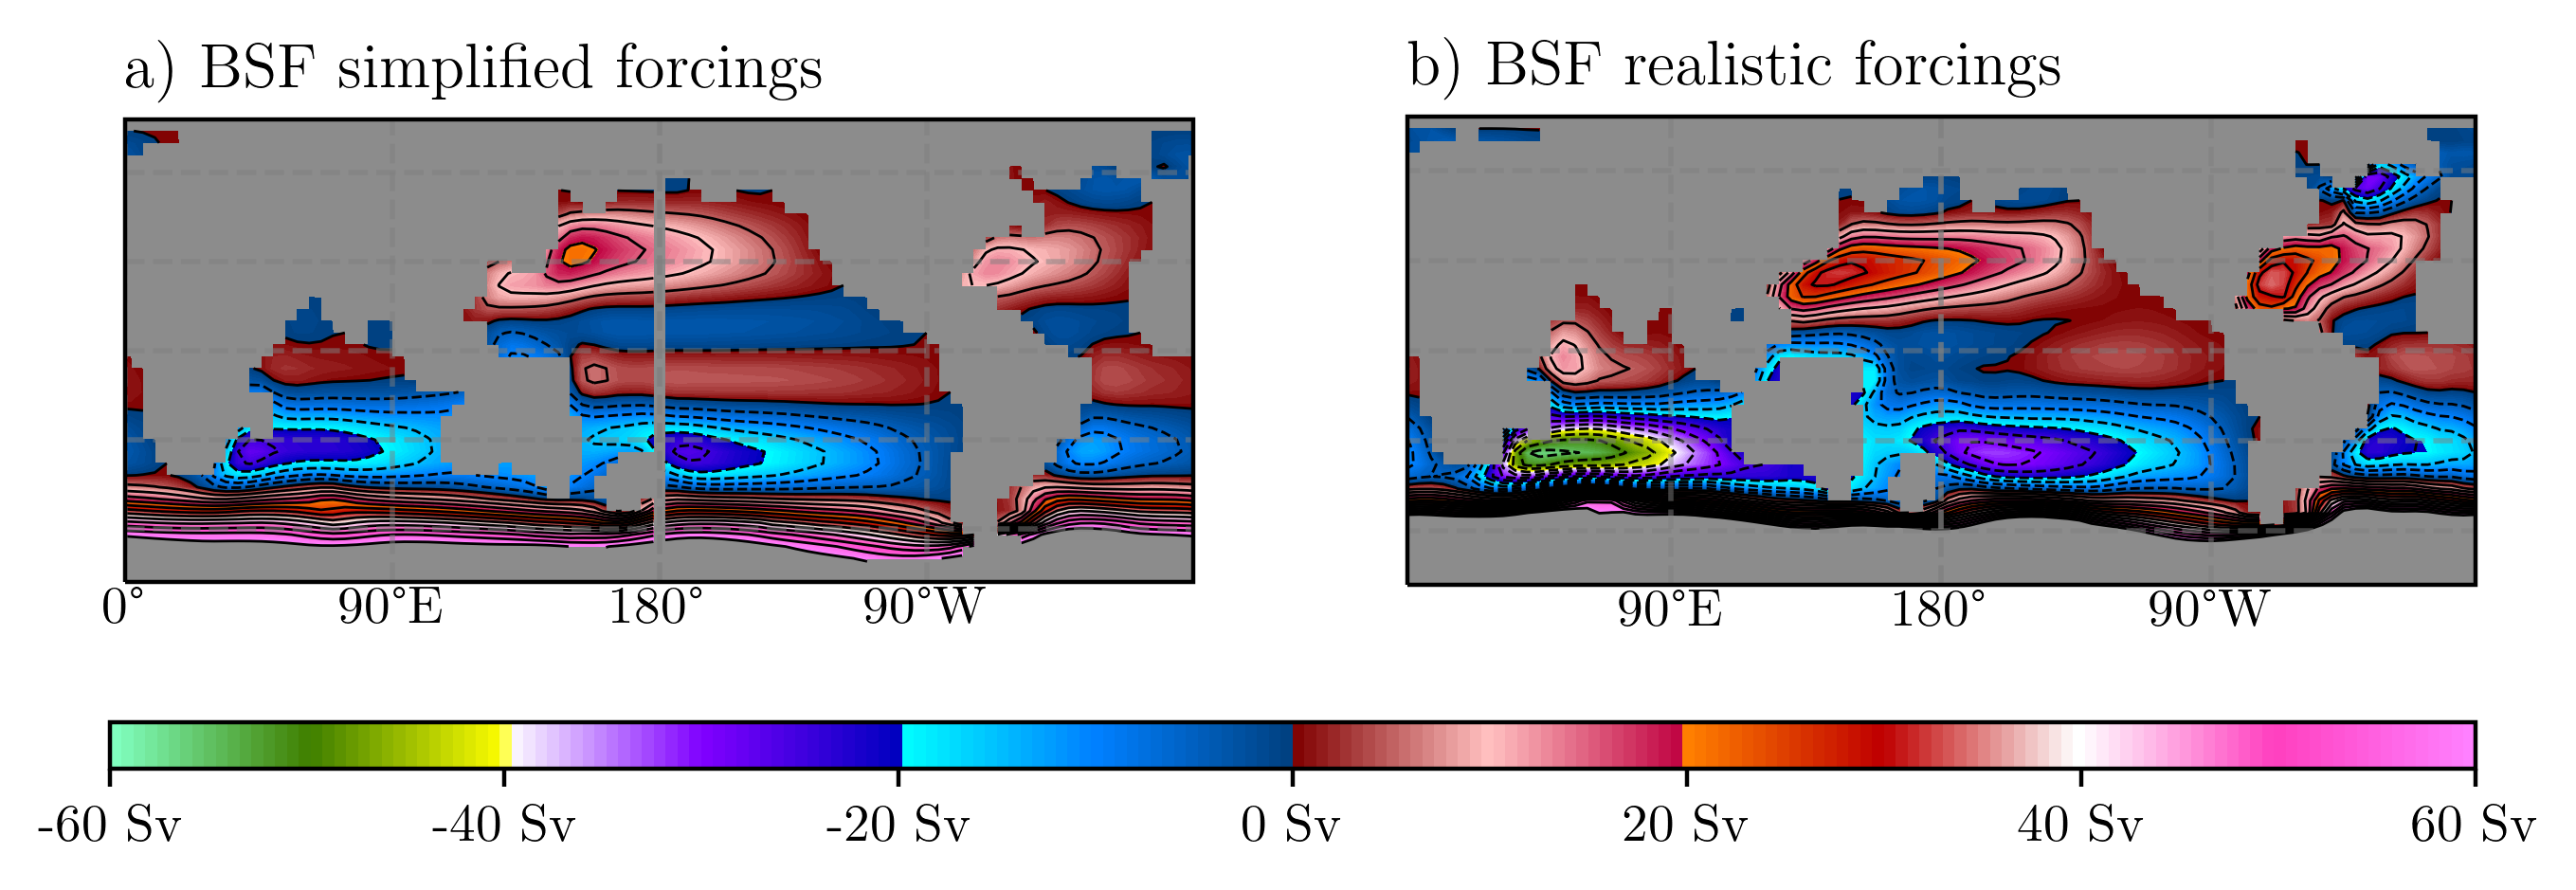
\includegraphics[width=\linewidth]{bsf_real_non.png}
\caption{Barotropic stream function with contours every 5 Sv. For \textbf{a)} simplified forcings and \textbf{b)} realistic forcings.}
\label{fig:bsf2_compared}
\end{figure}

\begin{multicols}{2}

\subsubsection{Quality of the MOC}
Next we look at the MOC stream functions and compare them between the two models. Here we must note the difference in geometry between the two models. This is due to the fact that we use an interpolated version in the simplified forcings case. That is different from the geometry used by Veros. In \cref{fig:moc_compared} we see the MOC stream function for the simplified and realistic models. Here the real problem of using simplified forcings is visible. The overturning circulation with the simplified forcings is extremely weak compared to the  overturning circulation with simplified forcings. We note that several key features are not captured by both models.

\todo[inline, color=green!40]{TODO: a piece on what is missing from the MOC. Mainly features discussed in the methods piece about the MOC}

\end{multicols}
\begin{figure}[H]
	
	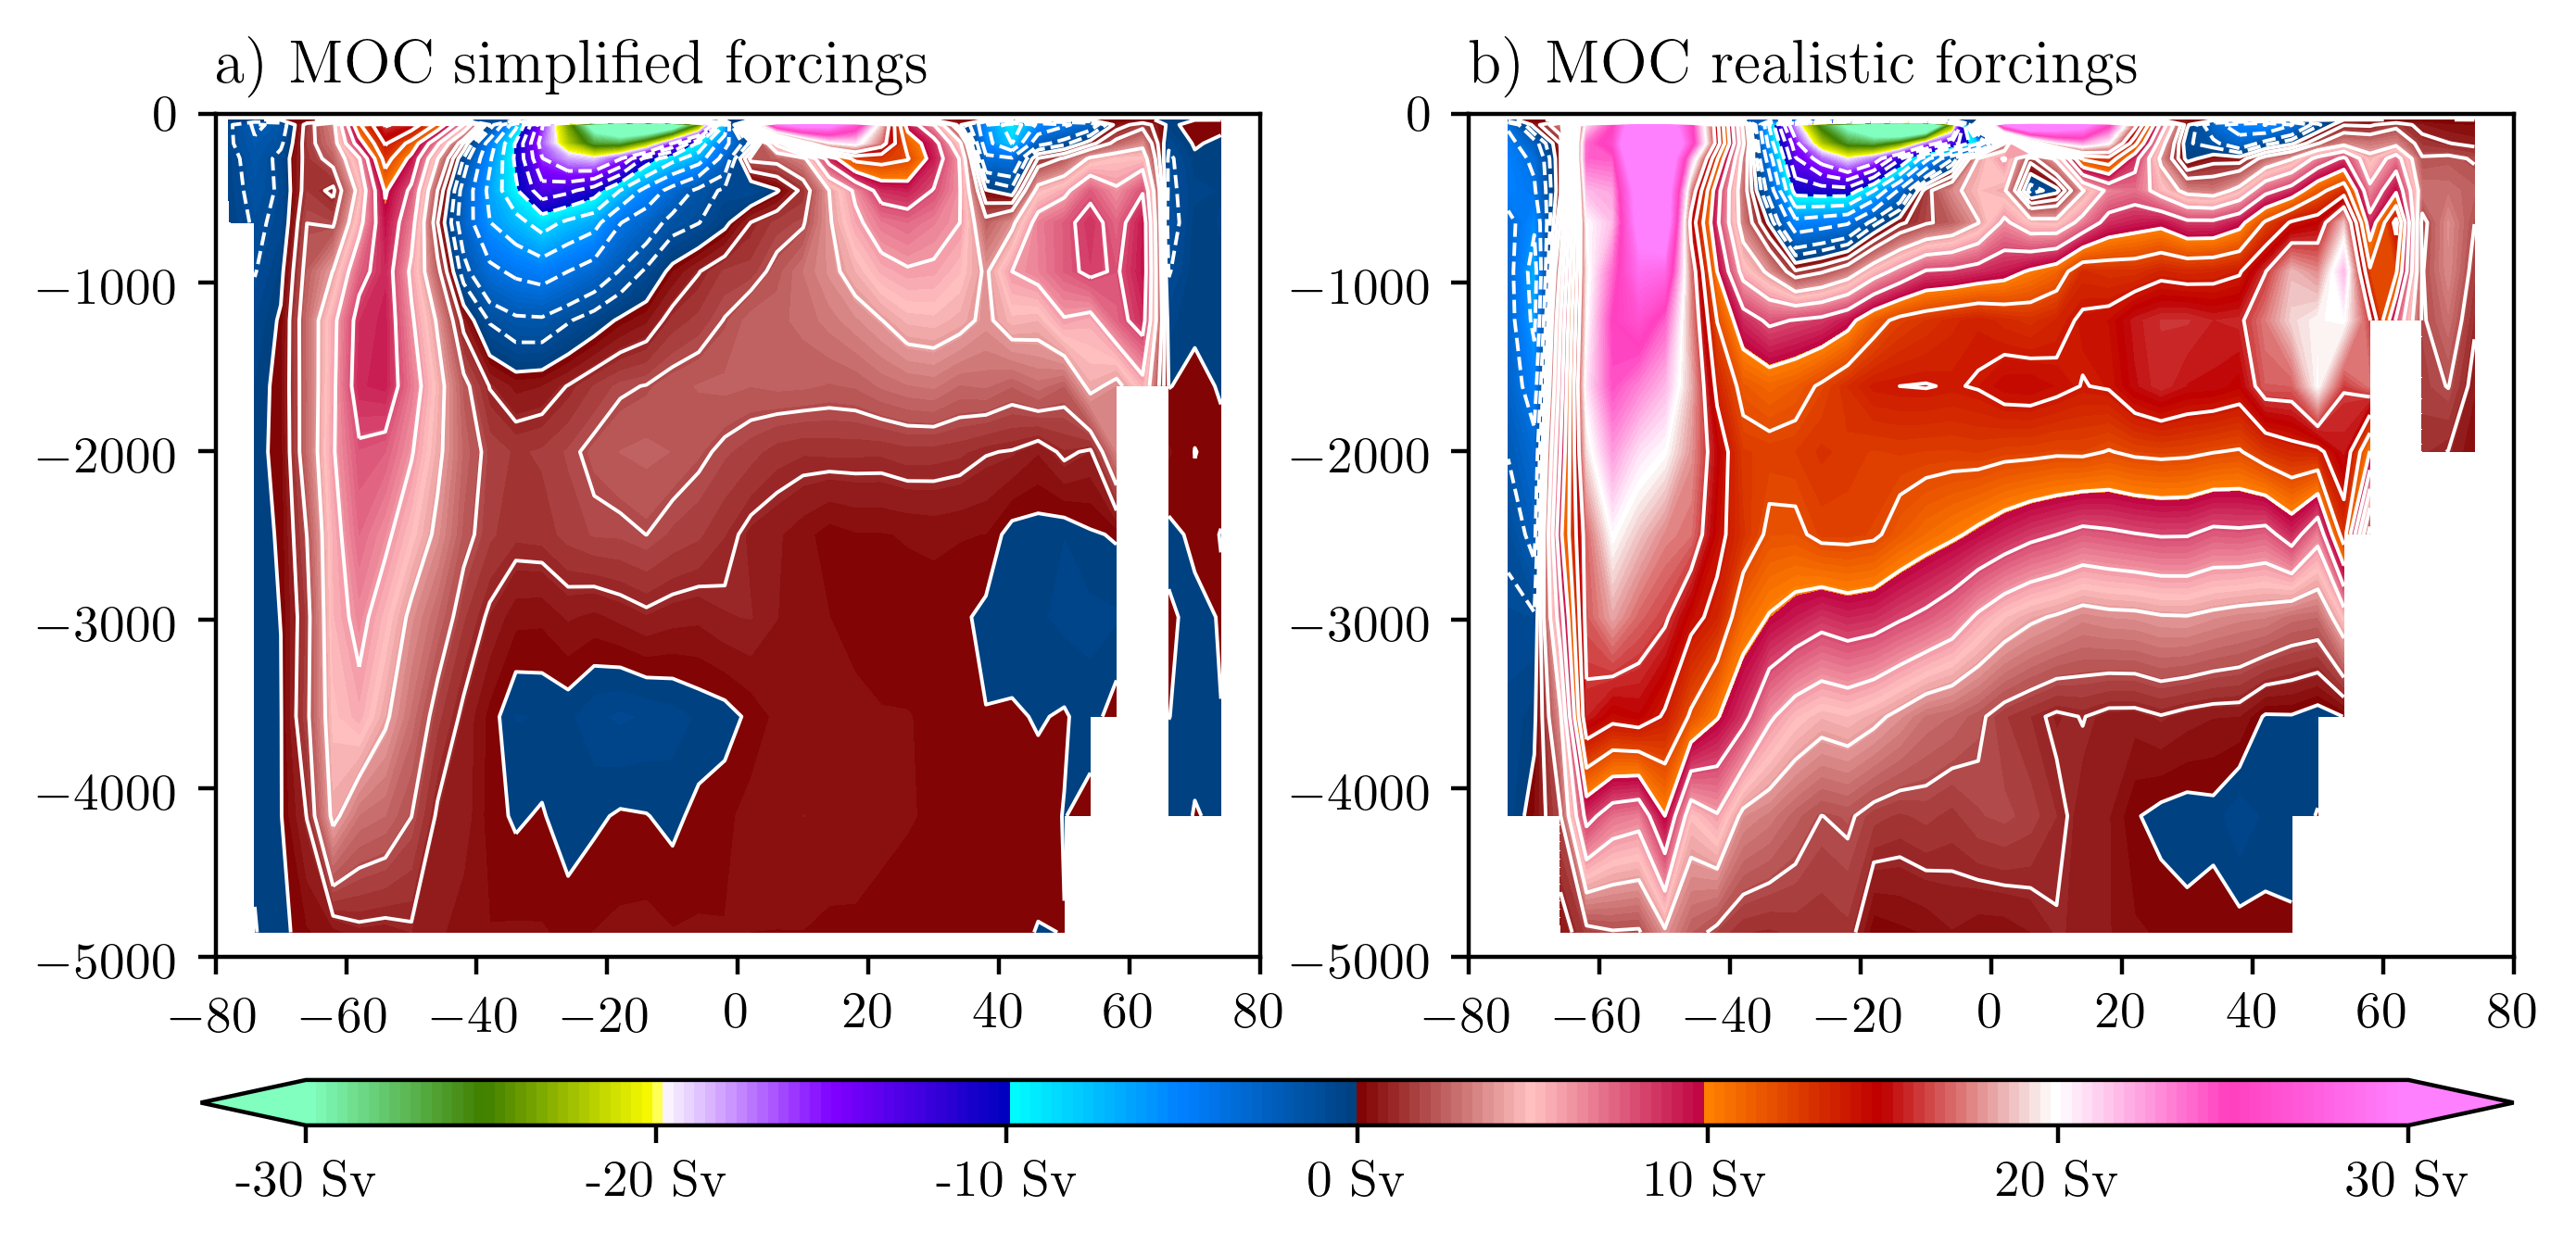
\includegraphics[width=\linewidth]{moc_forcings_real_fake.png}
	\caption{MOC stream function with contours every 2 Sv. For \textbf{a)} simplified forcings and \textbf{b)} realistic forcings. Negative values (dashed lines) indicate counterclockwise circulation}
	\label{fig:moc_compared}
\end{figure}

\begin{multicols}{2}
\subsubsection{Estimation of error}
\todo[inline, color=green!40]{TODO something on measuring the error introduced by the model. Probably by making a plot of the diffirence in MOC and the diffirence in BSF. And then extrapolate an error in Sv. Do not know if this is effective.}

\begin{figure}[H]
	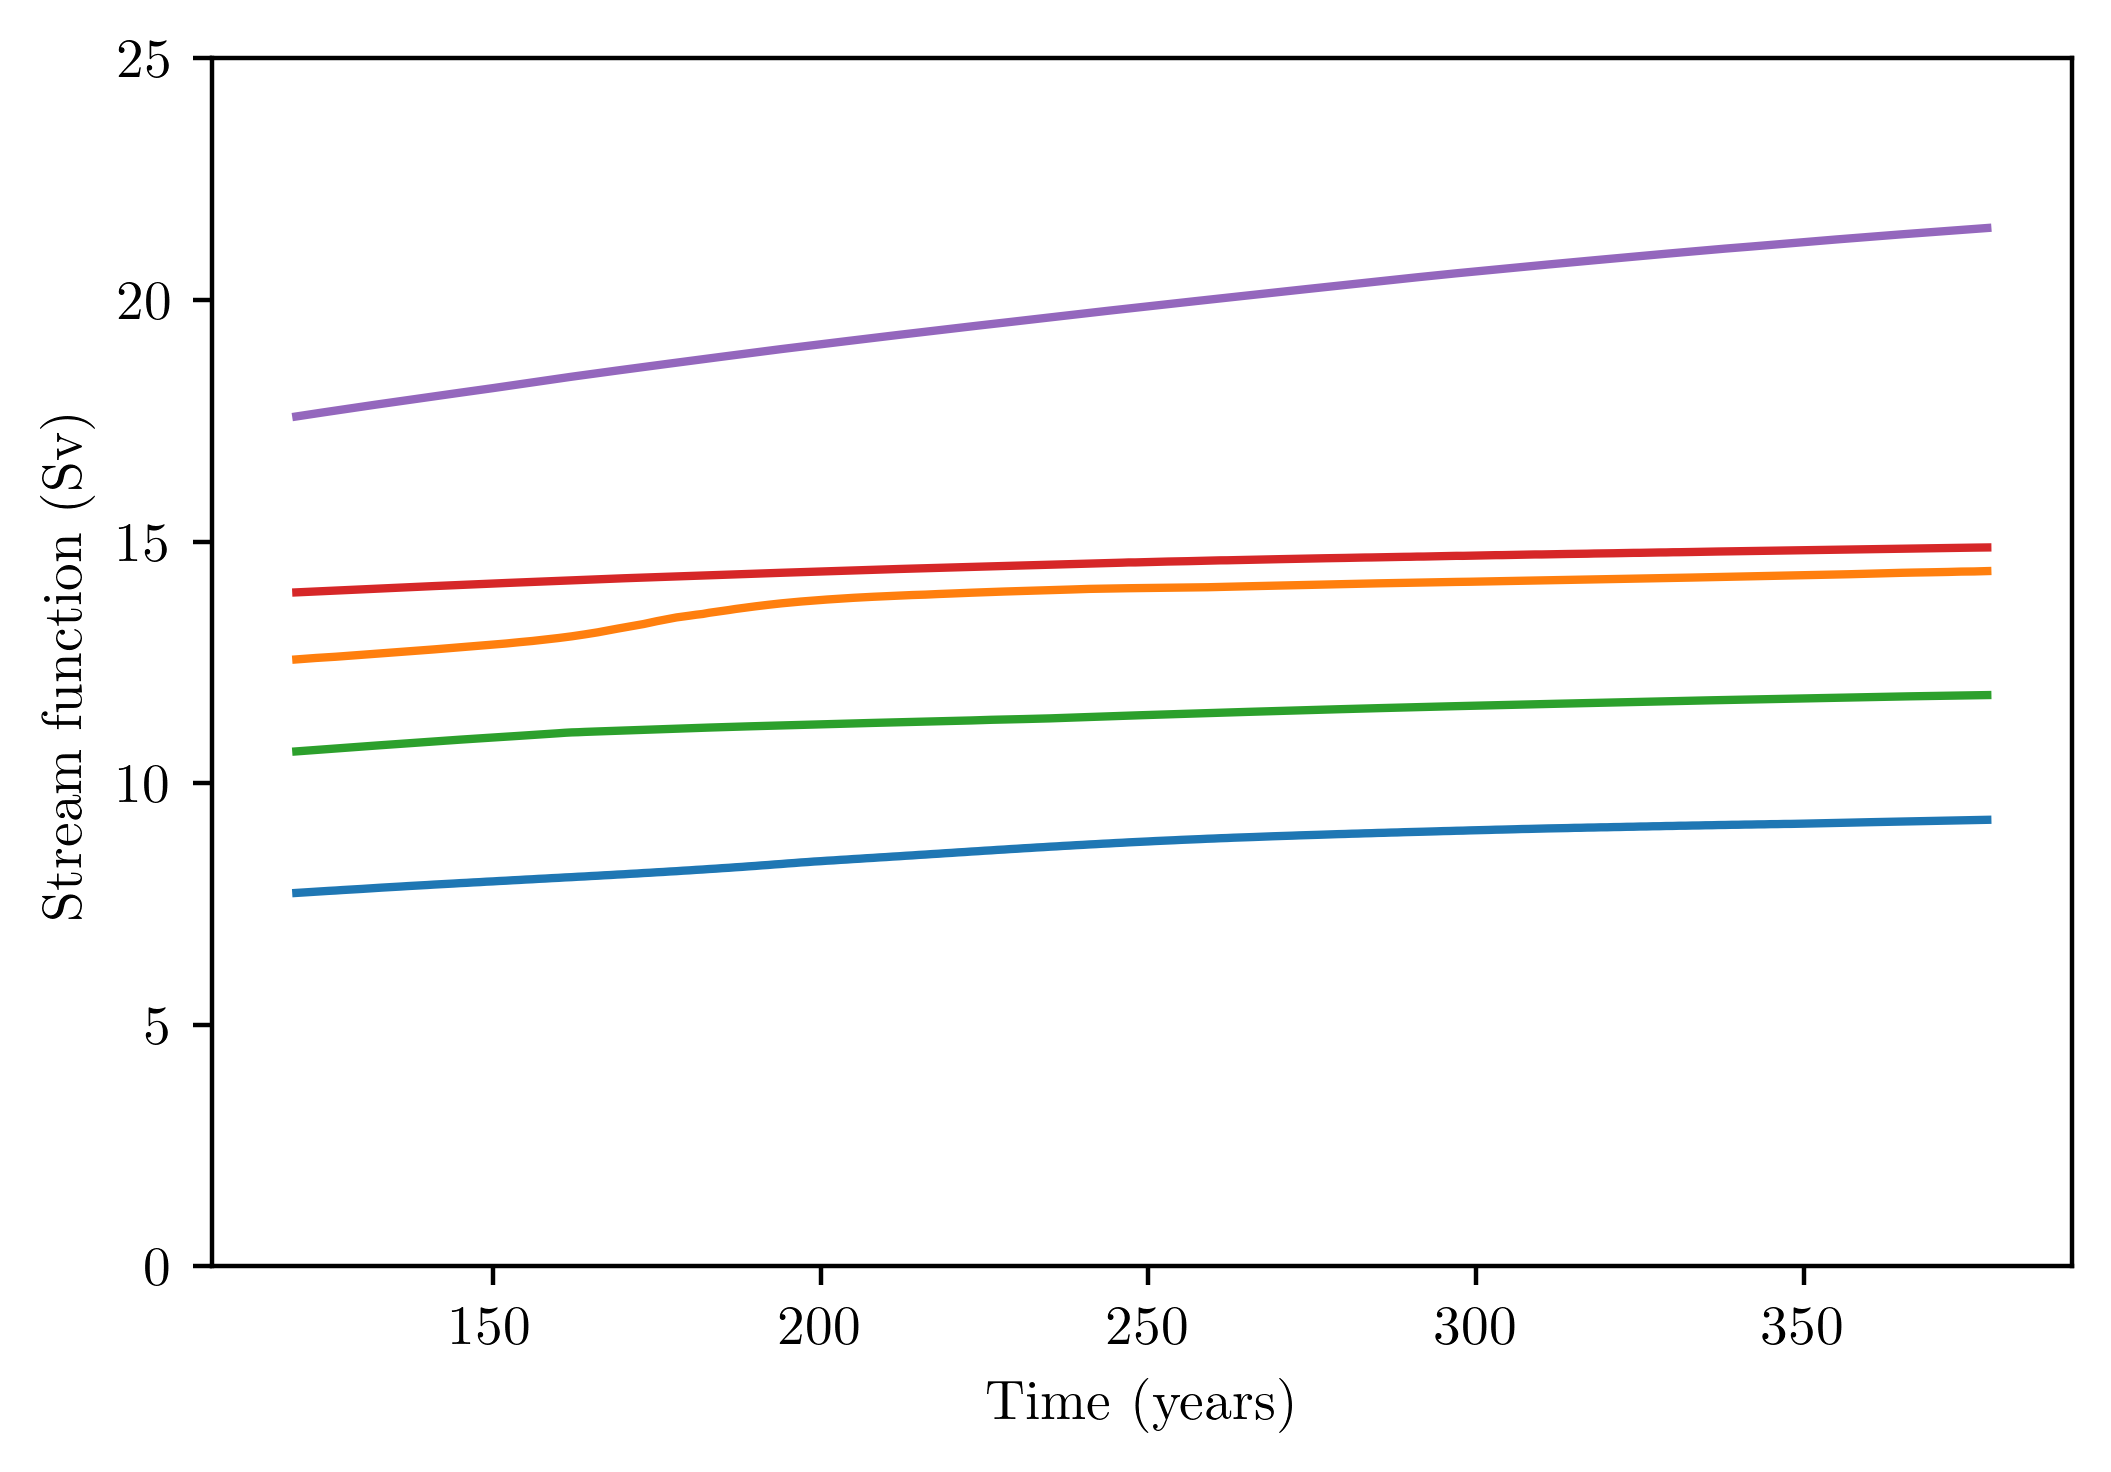
\includegraphics[width=\linewidth]{maxval_MOC.png}
	\caption{Maximum value of the MOC stream function in the northern hemisphere. Taken in the area $30^{\circ} - 80^{\circ}N$. Below $500m$.}
\end{figure}